% Options for packages loaded elsewhere
\PassOptionsToPackage{unicode}{hyperref}
\PassOptionsToPackage{hyphens}{url}
\PassOptionsToPackage{dvipsnames,svgnames,x11names}{xcolor}
%
\documentclass[
  letterpaper,
  DIV=11,
  numbers=noendperiod]{scrartcl}

\usepackage{amsmath,amssymb}
\usepackage{lmodern}
\usepackage{iftex}
\ifPDFTeX
  \usepackage[T1]{fontenc}
  \usepackage[utf8]{inputenc}
  \usepackage{textcomp} % provide euro and other symbols
\else % if luatex or xetex
  \usepackage{unicode-math}
  \defaultfontfeatures{Scale=MatchLowercase}
  \defaultfontfeatures[\rmfamily]{Ligatures=TeX,Scale=1}
\fi
% Use upquote if available, for straight quotes in verbatim environments
\IfFileExists{upquote.sty}{\usepackage{upquote}}{}
\IfFileExists{microtype.sty}{% use microtype if available
  \usepackage[]{microtype}
  \UseMicrotypeSet[protrusion]{basicmath} % disable protrusion for tt fonts
}{}
\makeatletter
\@ifundefined{KOMAClassName}{% if non-KOMA class
  \IfFileExists{parskip.sty}{%
    \usepackage{parskip}
  }{% else
    \setlength{\parindent}{0pt}
    \setlength{\parskip}{6pt plus 2pt minus 1pt}}
}{% if KOMA class
  \KOMAoptions{parskip=half}}
\makeatother
\usepackage{xcolor}
\setlength{\emergencystretch}{3em} % prevent overfull lines
\setcounter{secnumdepth}{-\maxdimen} % remove section numbering
% Make \paragraph and \subparagraph free-standing
\ifx\paragraph\undefined\else
  \let\oldparagraph\paragraph
  \renewcommand{\paragraph}[1]{\oldparagraph{#1}\mbox{}}
\fi
\ifx\subparagraph\undefined\else
  \let\oldsubparagraph\subparagraph
  \renewcommand{\subparagraph}[1]{\oldsubparagraph{#1}\mbox{}}
\fi

\usepackage{color}
\usepackage{fancyvrb}
\newcommand{\VerbBar}{|}
\newcommand{\VERB}{\Verb[commandchars=\\\{\}]}
\DefineVerbatimEnvironment{Highlighting}{Verbatim}{commandchars=\\\{\}}
% Add ',fontsize=\small' for more characters per line
\usepackage{framed}
\definecolor{shadecolor}{RGB}{241,243,245}
\newenvironment{Shaded}{\begin{snugshade}}{\end{snugshade}}
\newcommand{\AlertTok}[1]{\textcolor[rgb]{0.68,0.00,0.00}{#1}}
\newcommand{\AnnotationTok}[1]{\textcolor[rgb]{0.37,0.37,0.37}{#1}}
\newcommand{\AttributeTok}[1]{\textcolor[rgb]{0.40,0.45,0.13}{#1}}
\newcommand{\BaseNTok}[1]{\textcolor[rgb]{0.68,0.00,0.00}{#1}}
\newcommand{\BuiltInTok}[1]{\textcolor[rgb]{0.00,0.23,0.31}{#1}}
\newcommand{\CharTok}[1]{\textcolor[rgb]{0.13,0.47,0.30}{#1}}
\newcommand{\CommentTok}[1]{\textcolor[rgb]{0.37,0.37,0.37}{#1}}
\newcommand{\CommentVarTok}[1]{\textcolor[rgb]{0.37,0.37,0.37}{\textit{#1}}}
\newcommand{\ConstantTok}[1]{\textcolor[rgb]{0.56,0.35,0.01}{#1}}
\newcommand{\ControlFlowTok}[1]{\textcolor[rgb]{0.00,0.23,0.31}{#1}}
\newcommand{\DataTypeTok}[1]{\textcolor[rgb]{0.68,0.00,0.00}{#1}}
\newcommand{\DecValTok}[1]{\textcolor[rgb]{0.68,0.00,0.00}{#1}}
\newcommand{\DocumentationTok}[1]{\textcolor[rgb]{0.37,0.37,0.37}{\textit{#1}}}
\newcommand{\ErrorTok}[1]{\textcolor[rgb]{0.68,0.00,0.00}{#1}}
\newcommand{\ExtensionTok}[1]{\textcolor[rgb]{0.00,0.23,0.31}{#1}}
\newcommand{\FloatTok}[1]{\textcolor[rgb]{0.68,0.00,0.00}{#1}}
\newcommand{\FunctionTok}[1]{\textcolor[rgb]{0.28,0.35,0.67}{#1}}
\newcommand{\ImportTok}[1]{\textcolor[rgb]{0.00,0.46,0.62}{#1}}
\newcommand{\InformationTok}[1]{\textcolor[rgb]{0.37,0.37,0.37}{#1}}
\newcommand{\KeywordTok}[1]{\textcolor[rgb]{0.00,0.23,0.31}{#1}}
\newcommand{\NormalTok}[1]{\textcolor[rgb]{0.00,0.23,0.31}{#1}}
\newcommand{\OperatorTok}[1]{\textcolor[rgb]{0.37,0.37,0.37}{#1}}
\newcommand{\OtherTok}[1]{\textcolor[rgb]{0.00,0.23,0.31}{#1}}
\newcommand{\PreprocessorTok}[1]{\textcolor[rgb]{0.68,0.00,0.00}{#1}}
\newcommand{\RegionMarkerTok}[1]{\textcolor[rgb]{0.00,0.23,0.31}{#1}}
\newcommand{\SpecialCharTok}[1]{\textcolor[rgb]{0.37,0.37,0.37}{#1}}
\newcommand{\SpecialStringTok}[1]{\textcolor[rgb]{0.13,0.47,0.30}{#1}}
\newcommand{\StringTok}[1]{\textcolor[rgb]{0.13,0.47,0.30}{#1}}
\newcommand{\VariableTok}[1]{\textcolor[rgb]{0.07,0.07,0.07}{#1}}
\newcommand{\VerbatimStringTok}[1]{\textcolor[rgb]{0.13,0.47,0.30}{#1}}
\newcommand{\WarningTok}[1]{\textcolor[rgb]{0.37,0.37,0.37}{\textit{#1}}}

\providecommand{\tightlist}{%
  \setlength{\itemsep}{0pt}\setlength{\parskip}{0pt}}\usepackage{longtable,booktabs,array}
\usepackage{calc} % for calculating minipage widths
% Correct order of tables after \paragraph or \subparagraph
\usepackage{etoolbox}
\makeatletter
\patchcmd\longtable{\par}{\if@noskipsec\mbox{}\fi\par}{}{}
\makeatother
% Allow footnotes in longtable head/foot
\IfFileExists{footnotehyper.sty}{\usepackage{footnotehyper}}{\usepackage{footnote}}
\makesavenoteenv{longtable}
\usepackage{graphicx}
\makeatletter
\def\maxwidth{\ifdim\Gin@nat@width>\linewidth\linewidth\else\Gin@nat@width\fi}
\def\maxheight{\ifdim\Gin@nat@height>\textheight\textheight\else\Gin@nat@height\fi}
\makeatother
% Scale images if necessary, so that they will not overflow the page
% margins by default, and it is still possible to overwrite the defaults
% using explicit options in \includegraphics[width, height, ...]{}
\setkeys{Gin}{width=\maxwidth,height=\maxheight,keepaspectratio}
% Set default figure placement to htbp
\makeatletter
\def\fps@figure{htbp}
\makeatother

\KOMAoption{captions}{tableheading}
\makeatletter
\makeatother
\makeatletter
\makeatother
\makeatletter
\@ifpackageloaded{caption}{}{\usepackage{caption}}
\AtBeginDocument{%
\ifdefined\contentsname
  \renewcommand*\contentsname{Table of contents}
\else
  \newcommand\contentsname{Table of contents}
\fi
\ifdefined\listfigurename
  \renewcommand*\listfigurename{List of Figures}
\else
  \newcommand\listfigurename{List of Figures}
\fi
\ifdefined\listtablename
  \renewcommand*\listtablename{List of Tables}
\else
  \newcommand\listtablename{List of Tables}
\fi
\ifdefined\figurename
  \renewcommand*\figurename{Figure}
\else
  \newcommand\figurename{Figure}
\fi
\ifdefined\tablename
  \renewcommand*\tablename{Table}
\else
  \newcommand\tablename{Table}
\fi
}
\@ifpackageloaded{float}{}{\usepackage{float}}
\floatstyle{ruled}
\@ifundefined{c@chapter}{\newfloat{codelisting}{h}{lop}}{\newfloat{codelisting}{h}{lop}[chapter]}
\floatname{codelisting}{Listing}
\newcommand*\listoflistings{\listof{codelisting}{List of Listings}}
\makeatother
\makeatletter
\@ifpackageloaded{caption}{}{\usepackage{caption}}
\@ifpackageloaded{subcaption}{}{\usepackage{subcaption}}
\makeatother
\makeatletter
\@ifpackageloaded{tcolorbox}{}{\usepackage[many]{tcolorbox}}
\makeatother
\makeatletter
\@ifundefined{shadecolor}{\definecolor{shadecolor}{rgb}{.97, .97, .97}}
\makeatother
\makeatletter
\makeatother
\ifLuaTeX
  \usepackage{selnolig}  % disable illegal ligatures
\fi
\IfFileExists{bookmark.sty}{\usepackage{bookmark}}{\usepackage{hyperref}}
\IfFileExists{xurl.sty}{\usepackage{xurl}}{} % add URL line breaks if available
\urlstyle{same} % disable monospaced font for URLs
\hypersetup{
  colorlinks=true,
  linkcolor={blue},
  filecolor={Maroon},
  citecolor={Blue},
  urlcolor={Blue},
  pdfcreator={LaTeX via pandoc}}

\author{}
\date{}

\begin{document}
\ifdefined\Shaded\renewenvironment{Shaded}{\begin{tcolorbox}[sharp corners, boxrule=0pt, breakable, borderline west={3pt}{0pt}{shadecolor}, interior hidden, enhanced, frame hidden]}{\end{tcolorbox}}\fi

\renewcommand*\contentsname{Table of contents}
{
\hypersetup{linkcolor=}
\setcounter{tocdepth}{3}
\tableofcontents
}
\begin{Shaded}
\begin{Highlighting}[]
\ImportTok{from}\NormalTok{ frb\_ml\_utils }\ImportTok{import} \OperatorTok{*} 
\ImportTok{import}\NormalTok{ frb\_ml\_utils}
\ImportTok{import}\NormalTok{ numpy }\ImportTok{as}\NormalTok{ np}
\ImportTok{import}\NormalTok{ pandas }\ImportTok{as}\NormalTok{ pd}
\ImportTok{import}\NormalTok{ seaborn }\ImportTok{as}\NormalTok{ sns}
\ImportTok{import}\NormalTok{ scipy}
\ImportTok{import}\NormalTok{ sklearn}
\ImportTok{import}\NormalTok{ matplotlib.patches }\ImportTok{as}\NormalTok{ patches}
\ImportTok{from}\NormalTok{ matplotlib }\ImportTok{import}\NormalTok{ pyplot }\ImportTok{as}\NormalTok{ plt}
\ImportTok{from}\NormalTok{ sklearn }\ImportTok{import}\NormalTok{ svm}
\ImportTok{from}\NormalTok{ sklearn.tree }\ImportTok{import}\NormalTok{ DecisionTreeClassifier}
\ImportTok{from}\NormalTok{ sklearn.ensemble }\ImportTok{import}\NormalTok{ RandomForestClassifier,AdaBoostClassifier}
\ImportTok{from}\NormalTok{ sklearn.neighbors }\ImportTok{import}\NormalTok{ NearestCentroid}
\ImportTok{from}\NormalTok{ sklearn.metrics }\ImportTok{import}\NormalTok{ confusion\_matrix,ConfusionMatrixDisplay,accuracy\_score,f1\_score,roc\_auc\_score,balanced\_accuracy\_score,fbeta\_score}
\ImportTok{from}\NormalTok{ sklearn.model\_selection }\ImportTok{import}\NormalTok{ train\_test\_split}
\ImportTok{from}\NormalTok{ sklearn.inspection }\ImportTok{import}\NormalTok{ permutation\_importance}
\ImportTok{from}\NormalTok{ sklearn.preprocessing }\ImportTok{import}\NormalTok{ StandardScaler}
\ImportTok{from}\NormalTok{ imblearn.over\_sampling }\ImportTok{import}\NormalTok{ SMOTE}
\ImportTok{from}\NormalTok{ imblearn.pipeline }\ImportTok{import}\NormalTok{ Pipeline }\ImportTok{as}\NormalTok{ imbpipeline}
\ImportTok{from}\NormalTok{ xgboost }\ImportTok{import}\NormalTok{ XGBClassifier}
\ImportTok{from}\NormalTok{ lightgbm }\ImportTok{import}\NormalTok{ LGBMClassifier}
\ImportTok{from}\NormalTok{ dtreeviz.trees }\ImportTok{import}\NormalTok{ dtreeviz}
\ImportTok{from}\NormalTok{ dtreeviz }\ImportTok{import}\NormalTok{ clfviz}
\end{Highlighting}
\end{Shaded}

\begin{Shaded}
\begin{Highlighting}[]
\NormalTok{CHIME }\OperatorTok{=}\NormalTok{ load\_chime()}
\NormalTok{columns\_to\_use }\OperatorTok{=}\NormalTok{ [}\StringTok{\textquotesingle{}bc\_width\textquotesingle{}}\NormalTok{,}\StringTok{\textquotesingle{}flux\textquotesingle{}}\NormalTok{,}\StringTok{\textquotesingle{}fluence\textquotesingle{}}\NormalTok{,}\StringTok{\textquotesingle{}dm\_exc\_ne2001\textquotesingle{}}\NormalTok{,}
                  \StringTok{\textquotesingle{}peak\_freq\textquotesingle{}}\NormalTok{,}
                  \StringTok{\textquotesingle{}bright\_temp\textquotesingle{}}\NormalTok{,}\StringTok{\textquotesingle{}rest\_width\textquotesingle{}}\NormalTok{,}\StringTok{\textquotesingle{}freq\_width\textquotesingle{}}\NormalTok{,}\StringTok{\textquotesingle{}energy\textquotesingle{}}\NormalTok{]}

\NormalTok{CHIME[}\StringTok{\textquotesingle{}bright\_temp\textquotesingle{}}\NormalTok{] }\OperatorTok{=}\NormalTok{ np.log10(CHIME[}\StringTok{\textquotesingle{}bright\_temp\textquotesingle{}}\NormalTok{])}
\NormalTok{CHIME[}\StringTok{\textquotesingle{}energy\textquotesingle{}}\NormalTok{] }\OperatorTok{=}\NormalTok{ np.log10(CHIME[}\StringTok{\textquotesingle{}energy\textquotesingle{}}\NormalTok{])}
\NormalTok{CHIME[}\StringTok{\textquotesingle{}rest\_width\textquotesingle{}}\NormalTok{] }\OperatorTok{=}\NormalTok{ CHIME[}\StringTok{\textquotesingle{}rest\_width\textquotesingle{}}\NormalTok{] }\OperatorTok{*} \DecValTok{1000}
\NormalTok{CHIME[}\StringTok{\textquotesingle{}bc\_width\textquotesingle{}}\NormalTok{] }\OperatorTok{=}\NormalTok{ CHIME[}\StringTok{\textquotesingle{}bc\_width\textquotesingle{}}\NormalTok{] }\OperatorTok{*} \DecValTok{1000}

\NormalTok{CHIME[}\StringTok{\textquotesingle{}freq\_width\textquotesingle{}}\NormalTok{] }\OperatorTok{=}\NormalTok{ np.log10(CHIME[}\StringTok{\textquotesingle{}freq\_width\textquotesingle{}}\NormalTok{])}

\NormalTok{chime\_data }\OperatorTok{=}\NormalTok{ CHIME[columns\_to\_use]}
\NormalTok{chime\_target }\OperatorTok{=}\NormalTok{ (CHIME[}\StringTok{\textquotesingle{}repeater\_name\textquotesingle{}}\NormalTok{] }\OperatorTok{!=} \StringTok{\textquotesingle{}{-}9999\textquotesingle{}}\NormalTok{).to\_numpy().astype(}\StringTok{\textquotesingle{}int\textquotesingle{}}\NormalTok{)}
\NormalTok{X,test\_X,y,test\_y }\OperatorTok{=}\NormalTok{ train\_test\_split(chime\_data,chime\_target,test\_size}\OperatorTok{=}\FloatTok{0.3}\NormalTok{,stratify}\OperatorTok{=}\NormalTok{chime\_target)}

\NormalTok{scaler }\OperatorTok{=}\NormalTok{ StandardScaler()}
\NormalTok{scaler.fit(X)  }
\NormalTok{X }\OperatorTok{=}\NormalTok{ scaler.transform(X)  }
\NormalTok{test\_X }\OperatorTok{=}\NormalTok{ scaler.transform(test\_X)}
\NormalTok{chime\_data }\OperatorTok{=}\NormalTok{ scaler.transform(chime\_data)}

\NormalTok{X, y }\OperatorTok{=}\NormalTok{ SMOTE().fit\_resample(X, y)}
\end{Highlighting}
\end{Shaded}

\begin{verbatim}
2 78.8 0.00225301 FRB20180729A
12 101.5 0.00225301 FRB20180814A
38 101.0 0.00225301 FRB20180919A
49 94.7 0.00225301 FRB20180928A
75 101.3 0.00225301 FRB20181028A
76 101.3 0.00225301 FRB20181028A
77 101.3 0.00225301 FRB20181028A
78 101.3 0.00225301 FRB20181028A
79 101.3 0.00225301 FRB20181028A
81 62.3 0.00225301 FRB20181030A
82 62.5 0.00225301 FRB20181030B
158 83.6 0.00225301 FRB20181220A
174 92.6 0.00225301 FRB20181223C
221 96.1 0.00225301 FRB20190107B
399 100.8 0.00225301 FRB20190329A
459 79.4 0.00225301 FRB20190425A
571 100.7 0.00225301 FRB20190625E
572 100.7 0.00225301 FRB20190625E
573 100.7 0.00225301 FRB20190625E
576 101.5 0.00225301 FRB20190626A
\end{verbatim}

\begin{Shaded}
\begin{Highlighting}[]
\NormalTok{CHIME\_for\_plot }\OperatorTok{=}\NormalTok{ CHIME.copy()[columns\_to\_use]}
\NormalTok{CHIME\_for\_plot[}\StringTok{\textquotesingle{}Class\textquotesingle{}}\NormalTok{] }\OperatorTok{=}\NormalTok{ [}\StringTok{\textquotesingle{}Repeating\textquotesingle{}} \ControlFlowTok{if}\NormalTok{ row[}\StringTok{\textquotesingle{}repeater\_name\textquotesingle{}}\NormalTok{] }\OperatorTok{!=} \StringTok{\textquotesingle{}{-}9999\textquotesingle{}} \ControlFlowTok{else} \StringTok{\textquotesingle{}Non{-}repeating\textquotesingle{}} \ControlFlowTok{for}\NormalTok{ i,row }\KeywordTok{in}\NormalTok{ CHIME.iterrows()]}
\NormalTok{sns.set\_theme(}\StringTok{\textquotesingle{}paper\textquotesingle{}}\NormalTok{,}\StringTok{"ticks"}\NormalTok{,}\StringTok{\textquotesingle{}dark\textquotesingle{}}\NormalTok{)}
\NormalTok{sns.set\_context(}\StringTok{"paper"}\NormalTok{, rc}\OperatorTok{=}\NormalTok{\{}\StringTok{"font.size"}\NormalTok{:}\DecValTok{10}\NormalTok{,}\StringTok{"axes.labelsize"}\NormalTok{:}\DecValTok{18}\NormalTok{\})}
\NormalTok{p }\OperatorTok{=}\NormalTok{ sns.pairplot(pd.concat([CHIME\_for\_plot], axis}\OperatorTok{=}\DecValTok{1}\NormalTok{), hue}\OperatorTok{=}\StringTok{\textquotesingle{}Class\textquotesingle{}}\NormalTok{)}
\ControlFlowTok{for}\NormalTok{ ax }\KeywordTok{in}\NormalTok{ p.axes.flat:}
\NormalTok{    ax.tick\_params(axis}\OperatorTok{=}\StringTok{\textquotesingle{}both\textquotesingle{}}\NormalTok{, labelsize}\OperatorTok{=}\DecValTok{14}\NormalTok{)}
\NormalTok{p.legend.get\_title().set\_fontsize(}\DecValTok{15}\NormalTok{)}
\ControlFlowTok{for}\NormalTok{ legend\_text }\KeywordTok{in}\NormalTok{ p.legend.get\_texts():}
\NormalTok{    legend\_text.set\_fontsize(}\DecValTok{15}\NormalTok{)}
\NormalTok{p.tight\_layout()}
\CommentTok{\# plt.savefig(\textquotesingle{}./paper/features.pdf\textquotesingle{})}
\end{Highlighting}
\end{Shaded}

\begin{verbatim}
<seaborn.axisgrid.PairGrid at 0x203f203c850>
\end{verbatim}

\begin{figure}[H]

{\centering \includegraphics{frb-ml_files/figure-pdf/cell-4-output-2.png}

}

\end{figure}

\begin{Shaded}
\begin{Highlighting}[]
\NormalTok{clf }\OperatorTok{=}\NormalTok{ svm.SVC()}
\NormalTok{clf.fit(X, y)}
\NormalTok{predictions }\OperatorTok{=}\NormalTok{ clf.predict(test\_X)}
\BuiltInTok{print}\NormalTok{(predictions)}
\BuiltInTok{print}\NormalTok{(test\_y)}
\BuiltInTok{print}\NormalTok{(accuracy\_score(test\_y,predictions))}
\BuiltInTok{print}\NormalTok{(f1\_score(test\_y,predictions))}
\BuiltInTok{print}\NormalTok{(roc\_auc\_score(test\_y,predictions))}
\BuiltInTok{print}\NormalTok{(fbeta\_score(test\_y,predictions,beta}\OperatorTok{=}\DecValTok{2}\NormalTok{))}
\NormalTok{categories }\OperatorTok{=}\NormalTok{ [}\StringTok{\textquotesingle{}Non{-}repeating\textquotesingle{}}\NormalTok{, }\StringTok{\textquotesingle{}Repeating\textquotesingle{}}\NormalTok{]}
\NormalTok{cf }\OperatorTok{=}\NormalTok{ confusion\_matrix(test\_y, predictions)}
\NormalTok{make\_confusion\_matrix(cf, }
\NormalTok{                      categories}\OperatorTok{=}\NormalTok{categories,}
\NormalTok{                      cmap}\OperatorTok{=}\NormalTok{plt.cm.viridis,}
\NormalTok{                      figsize}\OperatorTok{=}\NormalTok{(}\DecValTok{5}\NormalTok{,}\DecValTok{4}\NormalTok{),}
\NormalTok{                      sum\_stats}\OperatorTok{=}\VariableTok{None}\NormalTok{)}
\CommentTok{\# plt.savefig(\textquotesingle{}./paper/svm\_cm.pdf\textquotesingle{})}
\end{Highlighting}
\end{Shaded}

\begin{verbatim}
[1 0 0 0 0 0 0 0 1 0 0 0 0 0 0 0 0 0 1 1 1 1 0 0 0 0 1 0 1 1 1 1 0 1 0 0 0
 0 0 1 0 0 0 1 1 0 0 0 0 0 1 0 0 1 0 0 1 1 0 1 0 0 1 1 0 0 0 0 0 0 0 0 0 0
 1 0 0 0 1 0 0 1 0 0 1 1 1 0 0 0 0 1 1 0 0 0 0 0 0 0 0 0 0 0 0 0 0 0 0 0 1
 0 0 0 0 0 0 0 0 0 0 1 0 0 0 0 0 1 1 0 0 0 0 0 0 0 0 0 0 0 0 0 0 0 0 1 1 1
 0 0 0 1 0 0 0 0 0 0 0 0 1 0 0 1 1 0 0 1 0 1 1 0 0 0 0 0 0 0 0]
[0 0 0 0 0 0 0 0 0 0 0 0 0 0 0 0 0 0 1 0 1 1 0 0 0 0 0 0 0 1 0 1 0 1 0 0 0
 0 0 1 0 0 0 1 0 0 0 0 0 0 0 0 0 0 0 0 1 1 0 0 0 1 1 0 0 0 0 0 0 0 0 0 0 0
 1 0 0 0 0 0 0 1 0 0 1 1 1 0 0 0 0 0 0 0 0 0 0 0 0 0 0 0 0 0 0 0 0 0 0 0 0
 0 0 0 0 0 0 0 0 0 0 1 0 0 0 0 0 1 0 0 0 0 0 0 0 0 0 0 0 1 0 1 0 0 0 1 1 1
 0 0 0 0 0 0 0 0 0 0 0 0 1 0 0 1 1 0 0 0 0 1 0 0 0 0 0 0 0 0 0]
0.8770949720670391
0.6944444444444445
0.8835146641438032
0.8012820512820514
\end{verbatim}

\begin{figure}[H]

{\centering \includegraphics{frb-ml_files/figure-pdf/cell-5-output-2.png}

}

\end{figure}

\begin{Shaded}
\begin{Highlighting}[]
\NormalTok{sns.set\_theme(}\StringTok{\textquotesingle{}paper\textquotesingle{}}\NormalTok{,}\StringTok{\textquotesingle{}ticks\textquotesingle{}}\NormalTok{)}
\NormalTok{result }\OperatorTok{=}\NormalTok{ permutation\_importance(clf, chime\_data, chime\_target, n\_repeats}\OperatorTok{=}\DecValTok{100}\NormalTok{, n\_jobs}\OperatorTok{={-}}\DecValTok{1}\NormalTok{,scoring}\OperatorTok{=}\NormalTok{f2\_score)}
\NormalTok{forest\_importances }\OperatorTok{=}\NormalTok{ pd.Series(result.importances\_mean, index}\OperatorTok{=}\NormalTok{columns\_to\_use)}

\NormalTok{fig, ax }\OperatorTok{=}\NormalTok{ plt.subplots()}
\NormalTok{forest\_importances.plot.bar(yerr}\OperatorTok{=}\NormalTok{result.importances\_std, ax}\OperatorTok{=}\NormalTok{ax,capsize}\OperatorTok{=}\DecValTok{4}\NormalTok{)}
\NormalTok{ax.set\_ylabel(}\VerbatimStringTok{r"Mean $F\_2$ decrease"}\NormalTok{)}
\NormalTok{fig.tight\_layout()}
\NormalTok{plt.show()}
\CommentTok{\# fig.savefig(\textquotesingle{}./paper/svm\_fi.pdf\textquotesingle{})}
\end{Highlighting}
\end{Shaded}

\begin{figure}[H]

{\centering \includegraphics{frb-ml_files/figure-pdf/cell-6-output-1.png}

}

\end{figure}

\begin{Shaded}
\begin{Highlighting}[]
\NormalTok{clf }\OperatorTok{=}\NormalTok{ RandomForestClassifier()}
\NormalTok{clf.fit(X, y)}
\NormalTok{predictions }\OperatorTok{=}\NormalTok{ clf.predict(test\_X)}
\BuiltInTok{print}\NormalTok{(predictions)}
\BuiltInTok{print}\NormalTok{(test\_y)}
\BuiltInTok{print}\NormalTok{(accuracy\_score(test\_y,predictions))}
\BuiltInTok{print}\NormalTok{(f1\_score(test\_y,predictions))}
\BuiltInTok{print}\NormalTok{(roc\_auc\_score(test\_y,predictions))}
\BuiltInTok{print}\NormalTok{(fbeta\_score(test\_y,predictions,beta}\OperatorTok{=}\DecValTok{2}\NormalTok{))}
\BuiltInTok{print}\NormalTok{(CHIME[np.logical\_and(clf.predict(chime\_data)}\OperatorTok{==}\DecValTok{1}\NormalTok{, chime\_target}\OperatorTok{==}\DecValTok{0}\NormalTok{)][}\StringTok{\textquotesingle{}tns\_name\textquotesingle{}}\NormalTok{])}
\NormalTok{categories }\OperatorTok{=}\NormalTok{ [}\StringTok{\textquotesingle{}Non{-}repeating\textquotesingle{}}\NormalTok{, }\StringTok{\textquotesingle{}Repeating\textquotesingle{}}\NormalTok{]}
\NormalTok{cf }\OperatorTok{=}\NormalTok{ confusion\_matrix(test\_y, predictions)}
\NormalTok{make\_confusion\_matrix(cf, }
\NormalTok{                      categories}\OperatorTok{=}\NormalTok{categories,}
\NormalTok{                      cmap}\OperatorTok{=}\NormalTok{plt.cm.viridis,}
\NormalTok{                      figsize}\OperatorTok{=}\NormalTok{(}\DecValTok{5}\NormalTok{,}\DecValTok{4}\NormalTok{),}
\NormalTok{                      sum\_stats}\OperatorTok{=}\VariableTok{None}\NormalTok{)}
\CommentTok{\# plt.savefig(\textquotesingle{}./paper/rf\_cm.pdf\textquotesingle{})}
\end{Highlighting}
\end{Shaded}

\begin{verbatim}
[0 0 0 0 0 0 0 0 0 0 0 0 0 0 0 0 0 0 0 0 1 1 0 0 0 0 1 0 1 1 1 1 0 1 0 0 0
 0 0 1 0 0 0 1 0 0 0 0 0 0 1 0 0 0 0 0 1 1 0 0 0 0 1 1 0 0 0 0 0 0 0 0 0 0
 1 0 0 0 1 0 0 0 0 0 1 1 1 0 0 0 0 0 0 0 0 0 0 0 0 0 0 0 0 0 0 0 0 0 0 0 1
 0 0 0 0 0 0 0 0 0 0 1 0 0 0 0 0 1 0 0 0 0 0 0 0 0 0 0 0 1 0 0 0 0 0 1 1 1
 0 0 0 0 0 0 0 0 0 0 0 0 1 0 0 1 1 0 0 0 0 1 0 0 0 0 0 0 0 0 0]
[0 0 0 0 0 0 0 0 0 0 0 0 0 0 0 0 0 0 1 0 1 1 0 0 0 0 0 0 0 1 0 1 0 1 0 0 0
 0 0 1 0 0 0 1 0 0 0 0 0 0 0 0 0 0 0 0 1 1 0 0 0 1 1 0 0 0 0 0 0 0 0 0 0 0
 1 0 0 0 0 0 0 1 0 0 1 1 1 0 0 0 0 0 0 0 0 0 0 0 0 0 0 0 0 0 0 0 0 0 0 0 0
 0 0 0 0 0 0 0 0 0 0 1 0 0 0 0 0 1 0 0 0 0 0 0 0 0 0 0 0 1 0 1 0 0 0 1 1 1
 0 0 0 0 0 0 0 0 0 0 0 0 1 0 0 1 1 0 0 0 0 1 0 0 0 0 0 0 0 0 0]
0.9385474860335196
0.8135593220338982
0.9053926206244087
0.8391608391608392
124    FRB20181128C
154    FRB20181218C
224    FRB20190109B
232    FRB20190112A
323    FRB20190218B
454    FRB20190423B
455    FRB20190423B
Name: tns_name, dtype: object
\end{verbatim}

\begin{figure}[H]

{\centering \includegraphics{frb-ml_files/figure-pdf/cell-7-output-2.png}

}

\end{figure}

\begin{Shaded}
\begin{Highlighting}[]
\NormalTok{sns.set\_theme(}\StringTok{\textquotesingle{}paper\textquotesingle{}}\NormalTok{,}\StringTok{\textquotesingle{}ticks\textquotesingle{}}\NormalTok{)}
\NormalTok{result }\OperatorTok{=}\NormalTok{ permutation\_importance(clf, chime\_data, chime\_target, n\_repeats}\OperatorTok{=}\DecValTok{100}\NormalTok{, n\_jobs}\OperatorTok{={-}}\DecValTok{1}\NormalTok{,scoring}\OperatorTok{=}\NormalTok{f2\_score)}
\NormalTok{forest\_importances }\OperatorTok{=}\NormalTok{ pd.Series(result.importances\_mean, index}\OperatorTok{=}\NormalTok{columns\_to\_use)}

\NormalTok{fig, ax }\OperatorTok{=}\NormalTok{ plt.subplots()}
\NormalTok{forest\_importances.plot.bar(yerr}\OperatorTok{=}\NormalTok{result.importances\_std, ax}\OperatorTok{=}\NormalTok{ax,capsize}\OperatorTok{=}\DecValTok{4}\NormalTok{)}
\NormalTok{ax.set\_ylabel(}\VerbatimStringTok{r"Mean $F\_2$ decrease"}\NormalTok{)}
\NormalTok{fig.tight\_layout()}
\NormalTok{plt.show()}
\CommentTok{\# fig.savefig(\textquotesingle{}./paper/rf\_fi.pdf\textquotesingle{})}
\end{Highlighting}
\end{Shaded}

\begin{figure}[H]

{\centering \includegraphics{frb-ml_files/figure-pdf/cell-8-output-1.png}

}

\end{figure}

\begin{Shaded}
\begin{Highlighting}[]
\NormalTok{clf }\OperatorTok{=}\NormalTok{ AdaBoostClassifier()}
\NormalTok{clf.fit(X, y)}
\NormalTok{predictions }\OperatorTok{=}\NormalTok{ clf.predict(test\_X)}
\BuiltInTok{print}\NormalTok{(predictions)}
\BuiltInTok{print}\NormalTok{(test\_y)}
\BuiltInTok{print}\NormalTok{(accuracy\_score(test\_y,predictions))}
\BuiltInTok{print}\NormalTok{(f1\_score(test\_y,predictions))}
\BuiltInTok{print}\NormalTok{(roc\_auc\_score(test\_y,predictions))}
\BuiltInTok{print}\NormalTok{(fbeta\_score(test\_y,predictions,beta}\OperatorTok{=}\DecValTok{2}\NormalTok{))}
\BuiltInTok{print}\NormalTok{(CHIME[np.logical\_and(clf.predict(chime\_data)}\OperatorTok{==}\DecValTok{1}\NormalTok{, chime\_target}\OperatorTok{==}\DecValTok{0}\NormalTok{)][}\StringTok{\textquotesingle{}tns\_name\textquotesingle{}}\NormalTok{])}
\NormalTok{categories }\OperatorTok{=}\NormalTok{ [}\StringTok{\textquotesingle{}Non{-}repeating\textquotesingle{}}\NormalTok{, }\StringTok{\textquotesingle{}Repeating\textquotesingle{}}\NormalTok{]}
\NormalTok{cf }\OperatorTok{=}\NormalTok{ confusion\_matrix(test\_y, predictions)}
\NormalTok{make\_confusion\_matrix(cf, }
\NormalTok{                      categories}\OperatorTok{=}\NormalTok{categories,}
\NormalTok{                      cmap}\OperatorTok{=}\NormalTok{plt.cm.viridis,}
\NormalTok{                      figsize}\OperatorTok{=}\NormalTok{(}\DecValTok{5}\NormalTok{,}\DecValTok{4}\NormalTok{),}
\NormalTok{                      sum\_stats}\OperatorTok{=}\VariableTok{None}\NormalTok{)}
\CommentTok{\# plt.savefig(\textquotesingle{}./paper/ab\_cm.pdf\textquotesingle{})}
\end{Highlighting}
\end{Shaded}

\begin{verbatim}
[0 0 0 0 0 0 0 0 0 0 0 0 0 0 0 0 0 0 1 1 1 1 0 0 0 0 1 0 1 0 1 1 0 1 0 0 0
 0 0 1 0 0 0 1 0 0 0 0 0 1 1 0 0 1 0 0 1 1 0 1 0 1 1 1 0 0 0 0 0 0 0 0 0 0
 1 0 0 0 1 0 0 1 0 0 1 1 1 0 0 0 0 0 0 0 0 0 0 0 0 1 0 0 0 0 0 0 0 0 0 0 1
 0 0 0 0 0 0 0 0 0 0 1 1 0 0 0 0 1 0 0 0 0 0 0 0 0 0 0 0 1 0 0 0 0 1 1 1 1
 0 0 0 1 0 0 0 0 0 0 0 0 1 0 0 1 1 0 0 0 0 1 1 0 0 0 0 0 0 0 0]
[0 0 0 0 0 0 0 0 0 0 0 0 0 0 0 0 0 0 1 0 1 1 0 0 0 0 0 0 0 1 0 1 0 1 0 0 0
 0 0 1 0 0 0 1 0 0 0 0 0 0 0 0 0 0 0 0 1 1 0 0 0 1 1 0 0 0 0 0 0 0 0 0 0 0
 1 0 0 0 0 0 0 1 0 0 1 1 1 0 0 0 0 0 0 0 0 0 0 0 0 0 0 0 0 0 0 0 0 0 0 0 0
 0 0 0 0 0 0 0 0 0 0 1 0 0 0 0 0 1 0 0 0 0 0 0 0 0 0 0 0 1 0 1 0 0 0 1 1 1
 0 0 0 0 0 0 0 0 0 0 0 0 1 0 0 1 1 0 0 0 0 1 0 0 0 0 0 0 0 0 0]
0.8994413407821229
0.742857142857143
0.9113055818353832
0.8441558441558441
2      FRB20180729A
40     FRB20180920B
84     FRB20181030E
99     FRB20181118B
115    FRB20181125A
117    FRB20181125A
124    FRB20181128C
125    FRB20181128C
154    FRB20181218C
174    FRB20181223C
196    FRB20181229B
203    FRB20181231B
224    FRB20190109B
232    FRB20190112A
272    FRB20190129A
291    FRB20190206B
323    FRB20190218B
349    FRB20190228A
418    FRB20190409B
421    FRB20190410A
449    FRB20190422A
450    FRB20190422A
454    FRB20190423B
455    FRB20190423B
Name: tns_name, dtype: object
\end{verbatim}

\begin{figure}[H]

{\centering \includegraphics{frb-ml_files/figure-pdf/cell-9-output-2.png}

}

\end{figure}

\begin{Shaded}
\begin{Highlighting}[]
\NormalTok{sns.set\_theme(}\StringTok{\textquotesingle{}paper\textquotesingle{}}\NormalTok{,}\StringTok{\textquotesingle{}ticks\textquotesingle{}}\NormalTok{)}
\CommentTok{\# result = permutation\_importance(clf, test\_X, test\_y, n\_repeats=100, n\_jobs={-}1,scoring=f2\_score)}
\NormalTok{result }\OperatorTok{=}\NormalTok{ permutation\_importance(clf, chime\_data, chime\_target, n\_repeats}\OperatorTok{=}\DecValTok{100}\NormalTok{, n\_jobs}\OperatorTok{={-}}\DecValTok{1}\NormalTok{,scoring}\OperatorTok{=}\NormalTok{f2\_score)}
\NormalTok{forest\_importances }\OperatorTok{=}\NormalTok{ pd.Series(result.importances\_mean, index}\OperatorTok{=}\NormalTok{columns\_to\_use)}

\NormalTok{fig, ax }\OperatorTok{=}\NormalTok{ plt.subplots()}
\NormalTok{forest\_importances.plot.bar(yerr}\OperatorTok{=}\NormalTok{result.importances\_std, ax}\OperatorTok{=}\NormalTok{ax,capsize}\OperatorTok{=}\DecValTok{4}\NormalTok{)}
\NormalTok{ax.set\_ylabel(}\VerbatimStringTok{r"Mean $F\_2$ decrease"}\NormalTok{)}
\NormalTok{fig.tight\_layout()}
\NormalTok{plt.show()}
\CommentTok{\# fig.savefig(\textquotesingle{}./paper/ab\_fi.pdf\textquotesingle{})}
\end{Highlighting}
\end{Shaded}

\begin{figure}[H]

{\centering \includegraphics{frb-ml_files/figure-pdf/cell-10-output-1.png}

}

\end{figure}

\begin{Shaded}
\begin{Highlighting}[]
\NormalTok{clf }\OperatorTok{=}\NormalTok{ NearestCentroid()}
\NormalTok{clf.fit(X, y)}
\NormalTok{predictions }\OperatorTok{=}\NormalTok{ clf.predict(test\_X)}
\BuiltInTok{print}\NormalTok{(predictions)}
\BuiltInTok{print}\NormalTok{(test\_y)}
\BuiltInTok{print}\NormalTok{(accuracy\_score(test\_y,predictions))}
\BuiltInTok{print}\NormalTok{(f1\_score(test\_y,predictions))}
\BuiltInTok{print}\NormalTok{(roc\_auc\_score(test\_y,predictions))}
\BuiltInTok{print}\NormalTok{(fbeta\_score(test\_y,predictions,beta}\OperatorTok{=}\DecValTok{2}\NormalTok{))}
\NormalTok{categories }\OperatorTok{=}\NormalTok{ [}\StringTok{\textquotesingle{}Non{-}repeating\textquotesingle{}}\NormalTok{, }\StringTok{\textquotesingle{}Repeating\textquotesingle{}}\NormalTok{]}
\NormalTok{cf }\OperatorTok{=}\NormalTok{ confusion\_matrix(test\_y, predictions)}
\NormalTok{make\_confusion\_matrix(cf, }
\NormalTok{                      categories}\OperatorTok{=}\NormalTok{categories,}
\NormalTok{                      cmap}\OperatorTok{=}\NormalTok{plt.cm.viridis,}
\NormalTok{                      figsize}\OperatorTok{=}\NormalTok{(}\DecValTok{5}\NormalTok{,}\DecValTok{4}\NormalTok{),}
\NormalTok{                      sum\_stats}\OperatorTok{=}\VariableTok{None}\NormalTok{)}
\CommentTok{\# plt.savefig(\textquotesingle{}./paper/nc\_cm.pdf\textquotesingle{})}
\end{Highlighting}
\end{Shaded}

\begin{verbatim}
[0 0 0 0 0 0 0 1 1 0 0 0 0 0 0 0 0 0 1 1 1 1 0 0 0 0 1 0 0 1 1 0 0 1 0 0 0
 0 0 1 0 1 0 1 0 0 0 0 0 0 0 0 0 1 0 0 1 1 0 1 0 0 1 1 0 0 0 0 0 1 0 0 0 0
 0 0 0 0 0 0 0 1 0 0 1 1 1 0 0 0 0 1 1 0 0 0 0 0 0 0 0 0 0 0 1 0 0 0 0 0 1
 0 0 0 0 0 0 0 0 0 0 1 1 0 0 1 0 1 0 0 0 0 0 0 0 0 0 0 0 0 0 1 0 0 1 1 1 1
 0 0 0 1 0 0 0 0 0 0 0 0 1 0 0 1 1 0 0 1 0 0 1 0 0 0 0 0 0 0 0]
[0 0 0 0 0 0 0 0 0 0 0 0 0 0 0 0 0 0 1 0 1 1 0 0 0 0 0 0 0 1 0 1 0 1 0 0 0
 0 0 1 0 0 0 1 0 0 0 0 0 0 0 0 0 0 0 0 1 1 0 0 0 1 1 0 0 0 0 0 0 0 0 0 0 0
 1 0 0 0 0 0 0 1 0 0 1 1 1 0 0 0 0 0 0 0 0 0 0 0 0 0 0 0 0 0 0 0 0 0 0 0 0
 0 0 0 0 0 0 0 0 0 0 1 0 0 0 0 0 1 0 0 0 0 0 0 0 0 0 0 0 1 0 1 0 0 0 1 1 1
 0 0 0 0 0 0 0 0 0 0 0 0 1 0 0 1 1 0 0 0 0 1 0 0 0 0 0 0 0 0 0]
0.8603351955307262
0.647887323943662
0.8444891201513718
0.7419354838709676
\end{verbatim}

\begin{figure}[H]

{\centering \includegraphics{frb-ml_files/figure-pdf/cell-11-output-2.png}

}

\end{figure}

\begin{Shaded}
\begin{Highlighting}[]
\NormalTok{sns.set\_theme(}\StringTok{\textquotesingle{}paper\textquotesingle{}}\NormalTok{,}\StringTok{\textquotesingle{}ticks\textquotesingle{}}\NormalTok{)}
\CommentTok{\# result = permutation\_importance(clf, test\_X, test\_y, n\_repeats=100, n\_jobs={-}1,scoring=f2\_score)}
\NormalTok{result }\OperatorTok{=}\NormalTok{ permutation\_importance(clf, chime\_data, chime\_target, n\_repeats}\OperatorTok{=}\DecValTok{100}\NormalTok{, n\_jobs}\OperatorTok{={-}}\DecValTok{1}\NormalTok{,scoring}\OperatorTok{=}\NormalTok{f2\_score)}
\NormalTok{forest\_importances }\OperatorTok{=}\NormalTok{ pd.Series(result.importances\_mean, index}\OperatorTok{=}\NormalTok{columns\_to\_use)}

\NormalTok{fig, ax }\OperatorTok{=}\NormalTok{ plt.subplots()}
\NormalTok{forest\_importances.plot.bar(yerr}\OperatorTok{=}\NormalTok{result.importances\_std, ax}\OperatorTok{=}\NormalTok{ax,capsize}\OperatorTok{=}\DecValTok{4}\NormalTok{)}
\NormalTok{ax.set\_ylabel(}\VerbatimStringTok{r"Mean $F\_2$ decrease"}\NormalTok{)}
\NormalTok{fig.tight\_layout()}
\NormalTok{plt.show()}
\CommentTok{\# fig.savefig(\textquotesingle{}./paper/nc\_fi.pdf\textquotesingle{})}
\end{Highlighting}
\end{Shaded}

\begin{figure}[H]

{\centering \includegraphics{frb-ml_files/figure-pdf/cell-12-output-1.png}

}

\end{figure}

\begin{Shaded}
\begin{Highlighting}[]
\NormalTok{clf }\OperatorTok{=}\NormalTok{ LGBMClassifier()}
\NormalTok{clf.fit(X, y)}
\NormalTok{predictions }\OperatorTok{=}\NormalTok{ clf.predict(test\_X)}
\BuiltInTok{print}\NormalTok{(predictions)}
\BuiltInTok{print}\NormalTok{(test\_y)}
\BuiltInTok{print}\NormalTok{(accuracy\_score(test\_y,predictions))}
\BuiltInTok{print}\NormalTok{(f1\_score(test\_y,predictions))}
\BuiltInTok{print}\NormalTok{(roc\_auc\_score(test\_y,predictions))}
\BuiltInTok{print}\NormalTok{(fbeta\_score(test\_y,predictions,beta}\OperatorTok{=}\DecValTok{2}\NormalTok{))}
\BuiltInTok{print}\NormalTok{(CHIME[np.logical\_and(clf.predict(chime\_data)}\OperatorTok{==}\DecValTok{1}\NormalTok{, chime\_target}\OperatorTok{==}\DecValTok{0}\NormalTok{)][}\StringTok{\textquotesingle{}tns\_name\textquotesingle{}}\NormalTok{])}
\NormalTok{categories }\OperatorTok{=}\NormalTok{ [}\StringTok{\textquotesingle{}Non{-}repeating\textquotesingle{}}\NormalTok{, }\StringTok{\textquotesingle{}Repeating\textquotesingle{}}\NormalTok{]}
\NormalTok{cf }\OperatorTok{=}\NormalTok{ confusion\_matrix(test\_y, predictions)}
\NormalTok{make\_confusion\_matrix(cf, }
\NormalTok{                      categories}\OperatorTok{=}\NormalTok{categories,}
\NormalTok{                      cmap}\OperatorTok{=}\NormalTok{plt.cm.viridis,}
\NormalTok{                      figsize}\OperatorTok{=}\NormalTok{(}\DecValTok{5}\NormalTok{,}\DecValTok{4}\NormalTok{),}
\NormalTok{                      sum\_stats}\OperatorTok{=}\VariableTok{None}\NormalTok{)}
\CommentTok{\# plt.savefig(\textquotesingle{}./paper/lgbm\_cm.pdf\textquotesingle{})}
\end{Highlighting}
\end{Shaded}

\begin{verbatim}
[0 0 0 0 0 0 0 0 0 0 0 0 0 0 0 0 0 0 0 0 1 1 0 0 0 0 1 0 1 0 1 1 0 1 0 0 0
 0 0 1 0 0 0 1 0 0 0 0 0 0 1 0 0 1 0 0 1 1 0 0 0 1 1 1 0 0 0 0 0 0 0 0 0 0
 1 0 0 0 0 0 0 1 0 0 1 1 1 0 0 0 0 0 1 0 0 0 0 0 0 0 0 0 0 0 0 0 0 0 0 0 0
 0 0 0 0 0 0 0 0 0 0 1 0 0 0 0 0 1 0 0 0 0 0 0 0 0 0 0 0 1 0 0 0 0 0 1 1 1
 0 0 0 0 0 0 0 0 0 0 0 0 1 0 0 1 1 0 0 0 0 1 0 0 0 0 0 0 0 0 0]
[0 0 0 0 0 0 0 0 0 0 0 0 0 0 0 0 0 0 1 0 1 1 0 0 0 0 0 0 0 1 0 1 0 1 0 0 0
 0 0 1 0 0 0 1 0 0 0 0 0 0 0 0 0 0 0 0 1 1 0 0 0 1 1 0 0 0 0 0 0 0 0 0 0 0
 1 0 0 0 0 0 0 1 0 0 1 1 1 0 0 0 0 0 0 0 0 0 0 0 0 0 0 0 0 0 0 0 0 0 0 0 0
 0 0 0 0 0 0 0 0 0 0 1 0 0 0 0 0 1 0 0 0 0 0 0 0 0 0 0 0 1 0 1 0 0 0 1 1 1
 0 0 0 0 0 0 0 0 0 0 0 0 1 0 0 1 1 0 0 0 0 1 0 0 0 0 0 0 0 0 0]
0.9441340782122905
0.8333333333333334
0.9232497634815515
0.8680555555555555
124    FRB20181128C
154    FRB20181218C
203    FRB20181231B
292    FRB20190206A
323    FRB20190218B
454    FRB20190423B
455    FRB20190423B
Name: tns_name, dtype: object
\end{verbatim}

\begin{figure}[H]

{\centering \includegraphics{frb-ml_files/figure-pdf/cell-13-output-2.png}

}

\end{figure}

\begin{Shaded}
\begin{Highlighting}[]
\NormalTok{sns.set\_theme(}\StringTok{\textquotesingle{}paper\textquotesingle{}}\NormalTok{,}\StringTok{\textquotesingle{}ticks\textquotesingle{}}\NormalTok{)}
\NormalTok{result }\OperatorTok{=}\NormalTok{ permutation\_importance(clf, chime\_data, chime\_target, n\_repeats}\OperatorTok{=}\DecValTok{100}\NormalTok{, n\_jobs}\OperatorTok{={-}}\DecValTok{1}\NormalTok{,scoring}\OperatorTok{=}\NormalTok{f2\_score)}
\NormalTok{forest\_importances }\OperatorTok{=}\NormalTok{ pd.Series(result.importances\_mean, index}\OperatorTok{=}\NormalTok{columns\_to\_use)}

\NormalTok{fig, ax }\OperatorTok{=}\NormalTok{ plt.subplots()}
\NormalTok{forest\_importances.plot.bar(yerr}\OperatorTok{=}\NormalTok{result.importances\_std, ax}\OperatorTok{=}\NormalTok{ax,capsize}\OperatorTok{=}\DecValTok{4}\NormalTok{)}
\NormalTok{ax.set\_ylabel(}\VerbatimStringTok{r"Mean $F\_2$ decrease"}\NormalTok{)}
\NormalTok{fig.tight\_layout()}
\NormalTok{plt.show()}
\CommentTok{\# fig.savefig(\textquotesingle{}./paper/lgbm\_fi.pdf\textquotesingle{})}
\end{Highlighting}
\end{Shaded}

\begin{figure}[H]

{\centering \includegraphics{frb-ml_files/figure-pdf/cell-14-output-1.png}

}

\end{figure}

\begin{Shaded}
\begin{Highlighting}[]
\NormalTok{clf }\OperatorTok{=}\NormalTok{ XGBClassifier(use\_label\_encoder}\OperatorTok{=}\VariableTok{False}\NormalTok{)}
\CommentTok{\# clf = CatBoostClassifier()}
\NormalTok{clf.fit(X, y)}
\NormalTok{predictions }\OperatorTok{=}\NormalTok{ clf.predict(test\_X)}
\BuiltInTok{print}\NormalTok{(predictions)}
\BuiltInTok{print}\NormalTok{(test\_y)}
\BuiltInTok{print}\NormalTok{(accuracy\_score(test\_y,predictions))}
\BuiltInTok{print}\NormalTok{(f1\_score(test\_y,predictions))}
\BuiltInTok{print}\NormalTok{(roc\_auc\_score(test\_y,predictions))}
\BuiltInTok{print}\NormalTok{(fbeta\_score(test\_y,predictions,beta}\OperatorTok{=}\DecValTok{2}\NormalTok{))}
\BuiltInTok{print}\NormalTok{(CHIME[np.logical\_and(clf.predict(chime\_data)}\OperatorTok{==}\DecValTok{1}\NormalTok{, chime\_target}\OperatorTok{==}\DecValTok{0}\NormalTok{)][}\StringTok{\textquotesingle{}tns\_name\textquotesingle{}}\NormalTok{])}
\NormalTok{categories }\OperatorTok{=}\NormalTok{ [}\StringTok{\textquotesingle{}Non{-}repeating\textquotesingle{}}\NormalTok{, }\StringTok{\textquotesingle{}Repeating\textquotesingle{}}\NormalTok{]}
\NormalTok{cf }\OperatorTok{=}\NormalTok{ confusion\_matrix(test\_y, predictions)}
\NormalTok{make\_confusion\_matrix(cf, }
\NormalTok{                      categories}\OperatorTok{=}\NormalTok{categories,}
\NormalTok{                      cmap}\OperatorTok{=}\NormalTok{plt.cm.viridis,}
\NormalTok{                      figsize}\OperatorTok{=}\NormalTok{(}\DecValTok{5}\NormalTok{,}\DecValTok{4}\NormalTok{),}
\NormalTok{                      sum\_stats}\OperatorTok{=}\VariableTok{None}\NormalTok{)}
\CommentTok{\# plt.savefig(\textquotesingle{}./paper/xgb\_cm.pdf\textquotesingle{})}
\end{Highlighting}
\end{Shaded}

\begin{verbatim}
d:\home\lab\sarjana\.venv\lib\site-packages\xgboost\sklearn.py:1421: UserWarning: `use_label_encoder` is deprecated in 1.7.0.
  warnings.warn("`use_label_encoder` is deprecated in 1.7.0.")
\end{verbatim}

\begin{verbatim}
[0 0 0 0 0 0 0 0 0 0 0 0 0 0 0 0 0 0 0 0 1 1 0 0 0 0 1 0 1 0 1 1 0 1 0 0 0
 0 0 1 0 0 0 1 0 0 0 0 0 0 1 0 0 1 0 0 1 1 0 0 0 1 1 1 0 0 0 0 0 0 0 0 0 0
 1 0 0 0 1 0 0 1 0 0 1 1 1 0 0 0 0 0 0 0 0 0 0 0 0 0 0 0 0 0 0 0 0 0 0 0 0
 0 0 0 0 0 0 0 0 0 0 1 1 0 0 0 0 1 0 0 0 0 0 0 0 0 0 0 0 1 0 0 0 0 0 1 1 1
 0 0 0 0 0 0 0 0 0 0 0 0 1 0 0 1 1 0 0 0 0 1 0 0 0 0 0 0 0 0 0]
[0 0 0 0 0 0 0 0 0 0 0 0 0 0 0 0 0 0 1 0 1 1 0 0 0 0 0 0 0 1 0 1 0 1 0 0 0
 0 0 1 0 0 0 1 0 0 0 0 0 0 0 0 0 0 0 0 1 1 0 0 0 1 1 0 0 0 0 0 0 0 0 0 0 0
 1 0 0 0 0 0 0 1 0 0 1 1 1 0 0 0 0 0 0 0 0 0 0 0 0 0 0 0 0 0 0 0 0 0 0 0 0
 0 0 0 0 0 0 0 0 0 0 1 0 0 0 0 0 1 0 0 0 0 0 0 0 0 0 0 0 1 0 1 0 0 0 1 1 1
 0 0 0 0 0 0 0 0 0 0 0 0 1 0 0 1 1 0 0 0 0 1 0 0 0 0 0 0 0 0 0]
0.9385474860335196
0.819672131147541
0.9199385052034058
0.8620689655172414
2      FRB20180729A
124    FRB20181128C
154    FRB20181218C
203    FRB20181231B
232    FRB20190112A
323    FRB20190218B
454    FRB20190423B
455    FRB20190423B
Name: tns_name, dtype: object
\end{verbatim}

\begin{figure}[H]

{\centering \includegraphics{frb-ml_files/figure-pdf/cell-15-output-3.png}

}

\end{figure}

\begin{Shaded}
\begin{Highlighting}[]
\NormalTok{sns.set\_theme(}\StringTok{\textquotesingle{}paper\textquotesingle{}}\NormalTok{,}\StringTok{\textquotesingle{}ticks\textquotesingle{}}\NormalTok{)}
\NormalTok{result }\OperatorTok{=}\NormalTok{ permutation\_importance(clf, chime\_data, chime\_target, n\_repeats}\OperatorTok{=}\DecValTok{100}\NormalTok{, n\_jobs}\OperatorTok{={-}}\DecValTok{1}\NormalTok{,scoring}\OperatorTok{=}\NormalTok{f2\_score)}
\NormalTok{forest\_importances }\OperatorTok{=}\NormalTok{ pd.Series(result.importances\_mean, index}\OperatorTok{=}\NormalTok{columns\_to\_use)}

\NormalTok{fig, ax }\OperatorTok{=}\NormalTok{ plt.subplots()}
\NormalTok{forest\_importances.plot.bar(yerr}\OperatorTok{=}\NormalTok{result.importances\_std, ax}\OperatorTok{=}\NormalTok{ax,capsize}\OperatorTok{=}\DecValTok{4}\NormalTok{)}
\NormalTok{ax.set\_ylabel(}\VerbatimStringTok{r"Mean $F\_2$ decrease"}\NormalTok{)}
\NormalTok{fig.tight\_layout()}
\NormalTok{plt.show()}
\CommentTok{\# fig.savefig(\textquotesingle{}./paper/xgb\_fi.pdf\textquotesingle{})}
\end{Highlighting}
\end{Shaded}

\begin{figure}[H]

{\centering \includegraphics{frb-ml_files/figure-pdf/cell-16-output-1.png}

}

\end{figure}

\begin{Shaded}
\begin{Highlighting}[]
\NormalTok{CHIME }\OperatorTok{=}\NormalTok{ load\_chime()}
\NormalTok{columns\_to\_use }\OperatorTok{=}\NormalTok{ [}\StringTok{\textquotesingle{}bc\_width\textquotesingle{}}\NormalTok{,}\StringTok{\textquotesingle{}flux\textquotesingle{}}\NormalTok{,}\StringTok{\textquotesingle{}fluence\textquotesingle{}}\NormalTok{,}\StringTok{\textquotesingle{}dm\_exc\_ne2001\textquotesingle{}}\NormalTok{,}
                  \StringTok{\textquotesingle{}peak\_freq\textquotesingle{}}\NormalTok{,}
                  \StringTok{\textquotesingle{}bright\_temp\textquotesingle{}}\NormalTok{,}\StringTok{\textquotesingle{}rest\_width\textquotesingle{}}\NormalTok{,}\StringTok{\textquotesingle{}freq\_width\textquotesingle{}}\NormalTok{,}\StringTok{\textquotesingle{}energy\textquotesingle{}}\NormalTok{]}
\NormalTok{CHIME[}\StringTok{\textquotesingle{}bright\_temp\textquotesingle{}}\NormalTok{] }\OperatorTok{=}\NormalTok{ np.log10(CHIME[}\StringTok{\textquotesingle{}bright\_temp\textquotesingle{}}\NormalTok{])}
\NormalTok{CHIME[}\StringTok{\textquotesingle{}energy\textquotesingle{}}\NormalTok{] }\OperatorTok{=}\NormalTok{ np.log10(CHIME[}\StringTok{\textquotesingle{}energy\textquotesingle{}}\NormalTok{])}
\NormalTok{CHIME[}\StringTok{\textquotesingle{}rest\_width\textquotesingle{}}\NormalTok{] }\OperatorTok{=}\NormalTok{ CHIME[}\StringTok{\textquotesingle{}rest\_width\textquotesingle{}}\NormalTok{] }\OperatorTok{*} \DecValTok{1000}
\NormalTok{CHIME[}\StringTok{\textquotesingle{}bc\_width\textquotesingle{}}\NormalTok{] }\OperatorTok{=}\NormalTok{ CHIME[}\StringTok{\textquotesingle{}bc\_width\textquotesingle{}}\NormalTok{] }\OperatorTok{*} \DecValTok{1000}
\NormalTok{CHIME[}\StringTok{\textquotesingle{}freq\_width\textquotesingle{}}\NormalTok{] }\OperatorTok{=}\NormalTok{ np.log10(CHIME[}\StringTok{\textquotesingle{}freq\_width\textquotesingle{}}\NormalTok{])}

\NormalTok{chime\_data }\OperatorTok{=}\NormalTok{ CHIME[columns\_to\_use]}
\NormalTok{chime\_target }\OperatorTok{=}\NormalTok{ (CHIME[}\StringTok{\textquotesingle{}repeater\_name\textquotesingle{}}\NormalTok{] }\OperatorTok{!=} \StringTok{\textquotesingle{}{-}9999\textquotesingle{}}\NormalTok{).to\_numpy().astype(}\StringTok{\textquotesingle{}int\textquotesingle{}}\NormalTok{)}
\NormalTok{X,test\_X,y,test\_y }\OperatorTok{=}\NormalTok{ train\_test\_split(chime\_data,chime\_target,test\_size}\OperatorTok{=}\FloatTok{0.3}\NormalTok{,stratify}\OperatorTok{=}\NormalTok{chime\_target)}

\NormalTok{X, y }\OperatorTok{=}\NormalTok{ SMOTE().fit\_resample(X, y)}
\NormalTok{clf }\OperatorTok{=}\NormalTok{ DecisionTreeClassifier(max\_depth}\OperatorTok{=}\DecValTok{5}\NormalTok{)  }
\NormalTok{clf.fit(X, y)}
\NormalTok{predictions }\OperatorTok{=}\NormalTok{ clf.predict(test\_X)}
\BuiltInTok{print}\NormalTok{(predictions)}
\BuiltInTok{print}\NormalTok{(test\_y)}
\BuiltInTok{print}\NormalTok{(accuracy\_score(test\_y,predictions))}
\BuiltInTok{print}\NormalTok{(f1\_score(test\_y,predictions))}
\BuiltInTok{print}\NormalTok{(roc\_auc\_score(test\_y,predictions))}
\BuiltInTok{print}\NormalTok{(fbeta\_score(test\_y,predictions,beta}\OperatorTok{=}\DecValTok{2}\NormalTok{))}
\NormalTok{categories }\OperatorTok{=}\NormalTok{ [}\StringTok{\textquotesingle{}Non{-}repeating\textquotesingle{}}\NormalTok{, }\StringTok{\textquotesingle{}Repeating\textquotesingle{}}\NormalTok{]}
\NormalTok{cf }\OperatorTok{=}\NormalTok{ confusion\_matrix(test\_y, predictions)}
\NormalTok{make\_confusion\_matrix(cf, }
\NormalTok{                      categories}\OperatorTok{=}\NormalTok{categories,}
\NormalTok{                      cmap}\OperatorTok{=}\NormalTok{plt.cm.viridis,}
\NormalTok{                      figsize}\OperatorTok{=}\NormalTok{(}\DecValTok{5}\NormalTok{,}\DecValTok{4}\NormalTok{),}
\NormalTok{                      sum\_stats}\OperatorTok{=}\VariableTok{None}\NormalTok{)}
\CommentTok{\# plt.savefig(\textquotesingle{}./paper/tree\_cm.pdf\textquotesingle{})}
\end{Highlighting}
\end{Shaded}

\begin{verbatim}
2 78.8 0.00225301 FRB20180729A
12 101.5 0.00225301 FRB20180814A
38 101.0 0.00225301 FRB20180919A
49 94.7 0.00225301 FRB20180928A
75 101.3 0.00225301 FRB20181028A
76 101.3 0.00225301 FRB20181028A
77 101.3 0.00225301 FRB20181028A
78 101.3 0.00225301 FRB20181028A
79 101.3 0.00225301 FRB20181028A
81 62.3 0.00225301 FRB20181030A
82 62.5 0.00225301 FRB20181030B
158 83.6 0.00225301 FRB20181220A
174 92.6 0.00225301 FRB20181223C
221 96.1 0.00225301 FRB20190107B
399 100.8 0.00225301 FRB20190329A
459 79.4 0.00225301 FRB20190425A
571 100.7 0.00225301 FRB20190625E
572 100.7 0.00225301 FRB20190625E
573 100.7 0.00225301 FRB20190625E
576 101.5 0.00225301 FRB20190626A
[1 0 0 0 0 0 1 0 0 0 1 0 0 0 1 0 0 0 0 0 1 1 0 1 1 0 0 0 1 0 1 0 0 1 0 0 1
 0 0 0 0 0 0 0 1 0 0 0 0 1 0 0 0 0 0 0 0 0 0 0 0 0 0 0 1 1 1 1 0 1 0 0 0 0
 0 0 0 1 1 0 0 0 0 0 1 0 0 0 1 1 0 1 0 0 0 1 1 0 0 0 0 0 0 0 0 0 0 1 0 0 0
 0 0 1 0 1 0 0 0 1 0 0 0 0 1 0 0 0 0 0 0 1 0 0 1 0 1 0 0 0 0 0 0 0 0 0 0 1
 0 0 0 0 1 0 0 0 0 1 1 0 1 0 1 0 0 0 0 0 0 0 1 0 0 0 0 0 0 1 0]
[0 0 0 0 0 0 0 0 0 0 1 0 0 0 1 1 0 0 0 0 0 1 0 0 0 0 0 0 1 0 0 0 0 1 0 0 0
 0 0 0 0 0 0 0 0 0 0 0 0 0 0 0 0 0 0 0 0 0 0 0 0 0 0 0 0 0 1 1 0 1 0 0 0 0
 0 0 0 1 0 0 0 0 0 0 1 0 0 0 0 1 0 0 0 0 0 1 0 0 0 0 0 0 0 0 0 0 0 0 0 0 0
 0 0 1 0 1 0 0 1 1 0 1 0 0 0 0 0 0 0 0 0 0 0 0 1 0 1 0 0 0 0 0 0 0 0 0 0 1
 0 0 0 0 1 0 0 0 0 1 0 0 1 0 1 0 0 0 0 0 0 0 1 0 1 0 0 0 0 1 0]
0.8715083798882681
0.676056338028169
0.8656575212866604
0.7741935483870968
\end{verbatim}

\begin{figure}[H]

{\centering \includegraphics{frb-ml_files/figure-pdf/cell-17-output-2.png}

}

\end{figure}

\begin{Shaded}
\begin{Highlighting}[]
\NormalTok{viz }\OperatorTok{=}\NormalTok{ dtreeviz(clf, chime\_data, chime\_target,feature\_names}\OperatorTok{=}\NormalTok{columns\_to\_use,class\_names}\OperatorTok{=}\NormalTok{[}\StringTok{\textquotesingle{}Non{-}repeating\textquotesingle{}}\NormalTok{,}\StringTok{\textquotesingle{}Repeating\textquotesingle{}}\NormalTok{],label\_fontsize}\OperatorTok{=}\DecValTok{18}\NormalTok{,ticks\_fontsize}\OperatorTok{=}\DecValTok{10}\NormalTok{)}
\NormalTok{viz}
\CommentTok{\# viz.save(\textquotesingle{}./paper/tree\_vis\_new.svg\textquotesingle{})}
\end{Highlighting}
\end{Shaded}

\begin{verbatim}
d:\home\lab\sarjana\.venv\lib\site-packages\sklearn\base.py:450: UserWarning: X does not have valid feature names, but DecisionTreeClassifier was fitted with feature names
  warnings.warn(
\end{verbatim}

\begin{figure}[H]

{\centering 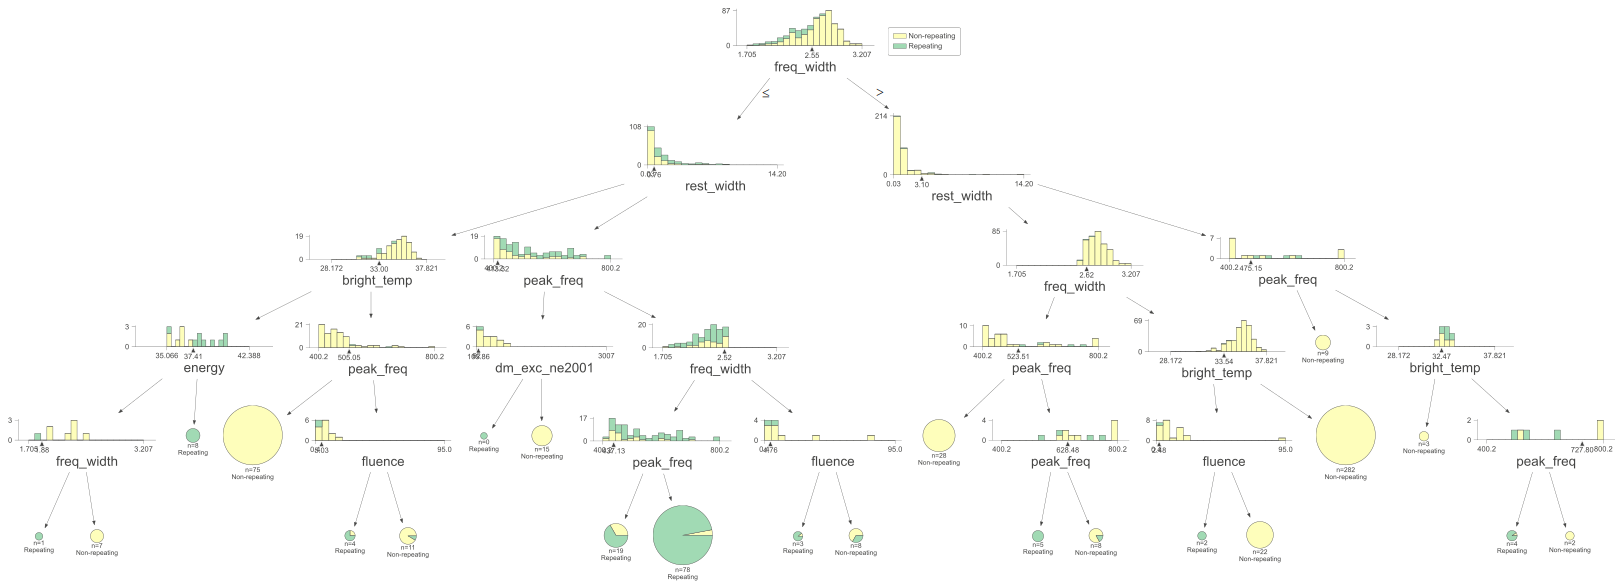
\includegraphics{frb-ml_files/figure-pdf/cell-18-output-2.svg}

}

\end{figure}

\begin{Shaded}
\begin{Highlighting}[]
\NormalTok{CHIME }\OperatorTok{=}\NormalTok{ load\_chime()}

\NormalTok{CHIME[}\StringTok{\textquotesingle{}bright\_temp\textquotesingle{}}\NormalTok{] }\OperatorTok{=}\NormalTok{ np.log10(CHIME[}\StringTok{\textquotesingle{}bright\_temp\textquotesingle{}}\NormalTok{])}
\NormalTok{CHIME[}\StringTok{\textquotesingle{}freq\_width\textquotesingle{}}\NormalTok{] }\OperatorTok{=}\NormalTok{ np.log10(CHIME[}\StringTok{\textquotesingle{}freq\_width\textquotesingle{}}\NormalTok{])}

\NormalTok{clf }\OperatorTok{=}\NormalTok{ imbpipeline(steps }\OperatorTok{=}\NormalTok{ [[}\StringTok{\textquotesingle{}scaler\textquotesingle{}}\NormalTok{, StandardScaler()],}
\NormalTok{                           [}\StringTok{\textquotesingle{}smote\textquotesingle{}}\NormalTok{, SMOTE()],}
\NormalTok{                           [}\StringTok{\textquotesingle{}classifier\textquotesingle{}}\NormalTok{, DecisionTreeClassifier(max\_depth}\OperatorTok{=}\DecValTok{3}\NormalTok{)]])}
\NormalTok{d2\_columns }\OperatorTok{=}\NormalTok{ [}\StringTok{\textquotesingle{}bright\_temp\textquotesingle{}}\NormalTok{,}\StringTok{\textquotesingle{}freq\_width\textquotesingle{}}\NormalTok{]}
\NormalTok{chime\_data\_2d }\OperatorTok{=}\NormalTok{ CHIME[d2\_columns]}
\NormalTok{X\_2d,test\_X\_2d,y\_2d,test\_y\_2d }\OperatorTok{=}\NormalTok{ train\_test\_split(chime\_data\_2d,chime\_target,test\_size}\OperatorTok{=}\FloatTok{0.3}\NormalTok{,stratify}\OperatorTok{=}\NormalTok{chime\_target)}
\NormalTok{clf.fit(X\_2d, y\_2d)}
\NormalTok{predictions }\OperatorTok{=}\NormalTok{ clf.predict(test\_X\_2d)}
\BuiltInTok{print}\NormalTok{(predictions)}
\BuiltInTok{print}\NormalTok{(test\_y\_2d)}
\BuiltInTok{print}\NormalTok{(accuracy\_score(test\_y\_2d,predictions))}
\BuiltInTok{print}\NormalTok{(f1\_score(test\_y\_2d,predictions))}
\BuiltInTok{print}\NormalTok{(roc\_auc\_score(test\_y\_2d,predictions))}
\BuiltInTok{print}\NormalTok{(fbeta\_score(test\_y\_2d,predictions,beta}\OperatorTok{=}\DecValTok{2}\NormalTok{))}
\NormalTok{categories }\OperatorTok{=}\NormalTok{ [}\StringTok{\textquotesingle{}Non{-}repeating\textquotesingle{}}\NormalTok{, }\StringTok{\textquotesingle{}Repeating\textquotesingle{}}\NormalTok{]}
\NormalTok{cf }\OperatorTok{=}\NormalTok{ confusion\_matrix(test\_y\_2d, predictions)}
\NormalTok{make\_confusion\_matrix(cf, }
\NormalTok{                      categories}\OperatorTok{=}\NormalTok{categories,}
\NormalTok{                      cmap}\OperatorTok{=}\NormalTok{plt.cm.viridis,}
\NormalTok{                      figsize}\OperatorTok{=}\NormalTok{(}\DecValTok{5}\NormalTok{,}\DecValTok{4}\NormalTok{),}
\NormalTok{                      sum\_stats}\OperatorTok{=}\VariableTok{None}\NormalTok{)}
\CommentTok{\# plt.savefig(\textquotesingle{}./paper/2d\_confusion.pdf\textquotesingle{})}

\NormalTok{fig,ax }\OperatorTok{=}\NormalTok{ plt.subplots(figsize}\OperatorTok{=}\NormalTok{(}\DecValTok{6}\NormalTok{,}\DecValTok{4}\NormalTok{))}
\NormalTok{clfviz(clf, chime\_data\_2d, chime\_target, ax}\OperatorTok{=}\NormalTok{ax, ntiles}\OperatorTok{=}\DecValTok{100}\NormalTok{,}
\NormalTok{       show}\OperatorTok{=}\NormalTok{[}\StringTok{\textquotesingle{}instances\textquotesingle{}}\NormalTok{, }\StringTok{\textquotesingle{}boundaries\textquotesingle{}}\NormalTok{, }\StringTok{\textquotesingle{}probabilities\textquotesingle{}}\NormalTok{, }\StringTok{\textquotesingle{}misclassified\textquotesingle{}}\NormalTok{],}
\NormalTok{       class\_names}\OperatorTok{=}\NormalTok{[}\StringTok{\textquotesingle{}non{-}repeating\textquotesingle{}}\NormalTok{,}\StringTok{\textquotesingle{}repeating\textquotesingle{}}\NormalTok{],}
\NormalTok{       feature\_names}\OperatorTok{=}\NormalTok{[}\StringTok{\textquotesingle{}log Brightness temperature (log K)\textquotesingle{}}\NormalTok{,}\StringTok{\textquotesingle{}log Frequency width (log MHz)\textquotesingle{}}\NormalTok{],}
\NormalTok{       colors}\OperatorTok{=}\NormalTok{\{}\StringTok{\textquotesingle{}class\_boundary\textquotesingle{}}\NormalTok{: }\StringTok{\textquotesingle{}red\textquotesingle{}}\NormalTok{,}\StringTok{\textquotesingle{}classes\textquotesingle{}}\NormalTok{:[}\VariableTok{None}\NormalTok{,  }\VariableTok{None}\NormalTok{,  [}\StringTok{"\#73ADD2"}\NormalTok{, }\StringTok{"\#FEE08F"}\NormalTok{]]\})}

\NormalTok{box1 }\OperatorTok{=}\NormalTok{ patches.Rectangle((}\DecValTok{0}\NormalTok{, }\DecValTok{0}\NormalTok{), }\DecValTok{20}\NormalTok{, }\DecValTok{10}\NormalTok{, linewidth}\OperatorTok{=}\FloatTok{.4}\NormalTok{, label}\OperatorTok{=}\StringTok{\textquotesingle{}Non{-}repeating\textquotesingle{}}\NormalTok{,edgecolor}\OperatorTok{=}\StringTok{\textquotesingle{}\#444443\textquotesingle{}}\NormalTok{,facecolor}\OperatorTok{=}\StringTok{\textquotesingle{}\#73ADD2\textquotesingle{}}\NormalTok{)}
\NormalTok{box2 }\OperatorTok{=}\NormalTok{ patches.Rectangle((}\DecValTok{0}\NormalTok{, }\DecValTok{0}\NormalTok{), }\DecValTok{20}\NormalTok{, }\DecValTok{10}\NormalTok{, linewidth}\OperatorTok{=}\FloatTok{.4}\NormalTok{, label}\OperatorTok{=}\StringTok{\textquotesingle{}Repeating\textquotesingle{}}\NormalTok{,edgecolor}\OperatorTok{=}\StringTok{\textquotesingle{}\#444443\textquotesingle{}}\NormalTok{,facecolor}\OperatorTok{=}\StringTok{\textquotesingle{}\#FEE08F\textquotesingle{}}\NormalTok{)}
\NormalTok{boxes }\OperatorTok{=}\NormalTok{ [box1,box2]}
\NormalTok{leg }\OperatorTok{=}\NormalTok{ ax.legend(handles}\OperatorTok{=}\NormalTok{boxes,frameon}\OperatorTok{=}\VariableTok{True}\NormalTok{,shadow}\OperatorTok{=}\VariableTok{False}\NormalTok{,fancybox}\OperatorTok{=}\VariableTok{True}\NormalTok{,handletextpad}\OperatorTok{=}\FloatTok{.35}\NormalTok{,borderpad}\OperatorTok{=}\FloatTok{.8}\NormalTok{,edgecolor}\OperatorTok{=}\StringTok{\textquotesingle{}\#444443\textquotesingle{}}\NormalTok{)}
\NormalTok{leg.get\_frame().set\_linewidth(}\FloatTok{.5}\NormalTok{)}
\NormalTok{plt.tight\_layout()}
\NormalTok{plt.show()}
\CommentTok{\# fig.savefig(\textquotesingle{}./paper/2d\_boundary.pdf\textquotesingle{})}
\end{Highlighting}
\end{Shaded}

\begin{verbatim}
2 78.8 0.00225301 FRB20180729A
12 101.5 0.00225301 FRB20180814A
38 101.0 0.00225301 FRB20180919A
49 94.7 0.00225301 FRB20180928A
75 101.3 0.00225301 FRB20181028A
76 101.3 0.00225301 FRB20181028A
77 101.3 0.00225301 FRB20181028A
78 101.3 0.00225301 FRB20181028A
79 101.3 0.00225301 FRB20181028A
81 62.3 0.00225301 FRB20181030A
82 62.5 0.00225301 FRB20181030B
158 83.6 0.00225301 FRB20181220A
174 92.6 0.00225301 FRB20181223C
221 96.1 0.00225301 FRB20190107B
399 100.8 0.00225301 FRB20190329A
459 79.4 0.00225301 FRB20190425A
571 100.7 0.00225301 FRB20190625E
572 100.7 0.00225301 FRB20190625E
573 100.7 0.00225301 FRB20190625E
576 101.5 0.00225301 FRB20190626A
[0 1 1 1 0 0 1 0 0 1 0 0 0 0 1 0 0 0 1 0 0 0 0 1 0 0 0 0 0 0 1 0 0 0 0 0 0
 0 0 0 0 0 1 0 0 1 1 1 0 1 1 1 0 1 0 0 0 1 0 1 1 0 1 1 1 0 0 0 0 0 0 0 1 1
 0 0 0 0 0 1 1 1 0 1 0 0 0 0 1 0 0 0 0 1 0 0 0 0 0 0 0 1 0 0 0 1 0 0 0 1 0
 1 0 1 1 0 0 0 1 1 1 0 1 1 0 0 0 1 0 1 0 0 0 0 0 0 1 0 1 1 0 0 0 0 1 1 0 0
 1 0 0 0 1 0 0 1 1 0 0 1 0 0 0 0 1 1 1 1 0 1 0 0 0 1 0 0 0 0 0]
[0 0 0 1 0 0 0 0 0 0 0 0 0 0 1 0 0 0 1 0 0 0 0 1 0 0 0 0 0 0 0 0 0 0 0 0 0
 0 0 0 0 0 0 0 0 0 0 1 0 0 1 0 0 0 1 0 0 1 0 1 1 0 0 0 0 0 0 0 0 0 0 0 0 1
 0 0 0 0 0 1 1 1 0 0 0 0 0 0 0 0 0 0 0 1 0 0 0 0 0 0 0 0 0 0 0 0 0 0 0 0 0
 0 0 1 1 0 0 0 1 1 0 0 1 1 0 0 0 1 0 1 0 0 0 0 0 0 0 0 0 1 0 0 0 0 0 0 0 0
 1 0 0 0 0 0 0 0 0 0 0 0 0 0 0 0 1 0 1 1 0 0 0 0 0 0 0 0 0 0 0]
0.8100558659217877
0.6136363636363636
0.8728713339640493
0.7848837209302326
\end{verbatim}

\begin{verbatim}
d:\home\lab\sarjana\.venv\lib\site-packages\sklearn\base.py:450: UserWarning: X does not have valid feature names, but StandardScaler was fitted with feature names
  warnings.warn(
d:\home\lab\sarjana\.venv\lib\site-packages\sklearn\base.py:450: UserWarning: X does not have valid feature names, but StandardScaler was fitted with feature names
  warnings.warn(
\end{verbatim}

\begin{figure}[H]

{\centering \includegraphics{frb-ml_files/figure-pdf/cell-19-output-3.png}

}

\end{figure}

\begin{figure}[H]

{\centering \includegraphics{frb-ml_files/figure-pdf/cell-19-output-4.png}

}

\end{figure}



\end{document}
